% THIS IS SIGPROC-SP.TEX - VERSION 3.1
% WORKS WITH V3.2SP OF ACM_PROC_ARTICLE-SP.CLS
% APRIL 2009
%
% It is an example file showing how to use the 'acm_proc_article-sp.cls' V3.2SP
% LaTeX2e document class file for Conference Proceedings submissions.
% ----------------------------------------------------------------------------------------------------------------
% This .tex file (and associated .cls V3.2SP) *DOES NOT* produce:
%       1) The Permission Statement
%       2) The Conference (location) Info information
%       3) The Copyright Line with ACM data
%       4) Page numbering
% ---------------------------------------------------------------------------------------------------------------
% It is an example which *does* use the .bib file (from which the .bbl file
% is produced).
% REMEMBER HOWEVER: After having produced the .bbl file,
% and prior to final submission,
% you need to 'insert'  your .bbl file into your source .tex file so as to provide
% ONE 'self-contained' source file
%
% Questions regarding SIGS should be sent to
% Adrienne Griscti ---> griscti@acm.org
%
% Questions/suggestions regarding the guidelines, .tex and .cls files, etc. to
% Gerald Murray ---> murray@hq.acm.org
%
% For tracking purposes - this is V3.1SP - APRIL 2009


\documentclass{acm_proc_article-sp}
%\documentclass{sig-alternate} 

\usepackage[utf8]{inputenc}
\usepackage{url}
\usepackage{float}
\usepackage{times}
\usepackage{color}
\usepackage{multirow}
\usepackage{listings}
\usepackage{times}
\usepackage{paralist}
\usepackage{wrapfig}
\usepackage{multirow}
\usepackage{ifpdf}
\usepackage{hyperref}
\usepackage[numbers, compress]{natbib}

\begin{document}

\conferenceinfo{ECMLS'12,} {}
\CopyrightYear{2012}
\crdata{978-1-4503-0702-4/11/06}
\clubpenalty=10000
\widowpenalty = 10000

\newif\ifdraft
%\drafttrue   
\ifdraft 
\newcommand{\jkimnote}[1]{{\textcolor{green} { ***Joohyun: #1 }}} 
\newcommand{\jhanote}[1]{ {\textcolor{red} { ***SJ: #1 }}}
\newcommand{\pmnote}[1]{ {\textcolor{red} { ***Pradeep: #1 }}}
\newcommand{\alnote}[1]{ {\textcolor{blue} { ***andreL: #1 }}}
\newcommand{\todo}[1]{ {\textcolor{red} { ***TODO: #1 }}}
\newcommand{\fix}[1]{ {\textcolor{red} { ***FIX: #1 }}}
\newcommand{\ny}[1]{ {\textcolor{red} { ***NY: #1 }}}
\newcommand{\reviewer}[1]{} 
\else 
\newcommand{\reviewer}[1]{}
\newcommand{\jkimnote}[1]{} 
\newcommand{\pmnote}[1]{}
\newcommand{\alnote}[1]{}
\newcommand{\jhanote}[1]{}
\newcommand{\todo}[1]{}
\fi


\title{Understanding MapReduce-based Next-Generation Sequencing
  Alignment on Distributed Cyberinfrastructure}

%\title{Next-Generation Sequencing Reads Alignment Using Pilot-based SAGA-MapReduce}

\numberofauthors{3} %  in this sample file, there are a *total*
% of EIGHT authors. SIX appear on the 'first-page' (for formatting
% reasons) and the remaining two appear in the \additionalauthors section.
%
\author{
% You can go ahead and credit any number of authors here,
% e.g. one 'row of three' or two rows (consisting of one row of three
% and a second row of one, two or three).
%
% The command \alignauthor (no curly braces needed) should
% precede each author name, affiliation/snail-mail address and
% e-mail address. Additionally, tag each line of
% affiliation/address with \affaddr, and tag the
% e-mail address with \email.
%
\alignauthor Pradeep Kumar Mantha\\
       \affaddr{Center for Computation and Technology}\\
       \affaddr{Louisiana State University}\\
       \affaddr{216 Johnston}\\
       \affaddr{Baton Rouge, LA}
       \email{pradeepm66@gmail.com}
\alignauthor Nayong Kim\\
       \affaddr{Center for Computation and Technology}\\
       \affaddr{Louisiana State University}\\
       \affaddr{216 Johnston}\\
       \affaddr{Baton Rouge, LA}
       \email{nykim@cct.lsu.edu}
\alignauthor Andre Luckow\\
       \affaddr{Center for Computation and Technology}\\
       \affaddr{Louisiana State University}\\
       \affaddr{216 Johnston}\\
       \affaddr{Baton Rouge, LA}
       \email{aluckow@cct.lsu.edu}
\and
\alignauthor Joohyun Kim\titlenote{Author for correspondence}\\
       \affaddr{Center for Computation and Technology}\\
       \affaddr{Louisiana State University}\\
       \affaddr{216 Johnston}\\
       \affaddr{Baton Rouge, LA} \\
       \email{jhkim@cct.lsu.edu}
\alignauthor Shantenu Jha\titlenote{Author for correspondence}\\
      \affaddr{Center for Computation and Technology}\\
     \affaddr{Louisiana State University}\\
      \affaddr{214 Johnston}\\
      \affaddr{Baton Rouge, LA}
     \email{sjha@cct.lsu.edu}
}
% There's nothing stopping you putting the seventh, eighth, etc.
% author on the opening page (as the 'third row') but we ask,
% for aesthetic reasons that you place these 'additional authors'
% in the \additional authors block, viz.
%\additionalauthors{Additional authors: John Smith (The Th{\o}rv{\"a}ld Group,
%email: {\texttt{jsmith@affiliation.org}}) and Julius P.~Kumquat
%(The Kumquat Consortium, email: {\texttt{jpkumquat@consortium.net}}).}
\date{25 Feb. 2012}
% Just remember to make sure that the TOTAL number of authors
% is the number that will appear on the first page PLUS the
% number that will appear in the \additionalauthors section.

\maketitle
\begin{abstract} 
  Although localization of Next-Generation Sequencing (NGS) data is
  suitable for many analysis and usage scenarios, it is not
  universally desirable, nor possible. However most solutions
  ``impose'' the localization of data as a pre-condition for NGS
  analytics.  We analyze several existing tools and techniques that
  use MapReduce programming model for NGS
  data analysis to determine their effectiveness and extensibility to
  support distributed data scenarios. We find limitations at multiple
  levels. To overcome these limitations, we developed a Pilot-based
  MapReduce (PMR) -- which is a novel implementation of MapReduce
  using a Pilot task and data management implementation.  PMR provides
  an effective means by which a variety of new or existing methods for
  NGS and downstream analysis can be carried out whilst providing
  efficiency and scalability across multiple clusters.  We compare and
  contrast the PMR approach to similar capabilities of SEQAL and
  Crossbow, two other tools which are based on conventional
  Hadoop-based MapReduce for NGS reads alignment and duplicate removal
  or SNP finding, respectively. We find that PMR is a viable tool to
  support distributed NGS analytics, as well as providing a framework
  that supports parallelism at multiple levels. % -- fine grained
  % task-level concurrency for a wide range of NGS data analysis and
  % downstream processing.
\end{abstract}

% We analyze several existing tools and technqiues that use MapReduce
% programming model for Next-Generatiion Sequencing (NGS) data analysis.
% Our approach is based on the Pilot-based SAGA-MapReduce (PMR)
% framework which extends previously introduced SAGA-MapReduce with a
% Pilot task and data management implementation.  PMR provides an
% effective means to develop software tools with which a variety of
% existing or novel methods for NGS data and downstream analysis are
% carried out and more importantly achieve scalability across multiple
% clusters.  As demonstrating examples for the capabilities of our
% PMR-based approach, we implemented similar capabilities of SEQAL and
% Crossbow, two other tools which are based on conventional Hadoop-based
% MapReduce for NGS reads alignment and duplicate removal or SNP
% finding, respectively.  The comparison to these tools allows us to
% characterize our approach with PMR as a viable tool for the
% scale-across requirement as well as a versatile parallelism framework
% for a wide range of NGS data analysis and process tools.  The
% scalability with distributed sequencing data and the potentials for
% other analysis applications are discussed.


\category{D.1.3}{Software}{Concurrent Programming}{ Distributed
  programming/parallel programming} \category{J.3}{Computer
  Applications}{Bioinformatics, Mapping}


% A category with the (minimum) three required fields
%\category{H.4}{Information Systems Applications}{Miscellaneous} %Acategory including the fourth, optional field follows...
%\category{D.2.8}{Software Engineering}{Metrics}[complexity measures,performance measures]

\terms{Design, Experimentation, Performance}

 \keywords{Genome Sequence Alignment, BWA, Human Genome, RNA-Seq Data,
  MapReduce, Distributed Computing, Simple API for Grid
  Applications (SAGA), Pilot Job and Data}

%\keywords{ACM proceedings, \LaTeX, text tagging} % NOT required for Proceedings 
%\keywords{RNA conformation energy landscape, Runtime Environment, SAM-I riboswitch,
% S gene of Bovine Corona Viral Genome} % NOT required for Proceedings


% With astronomically explosive volumes of raw data and processed data,
% along with computational tasks that often need scalable
% infrastructure,
% computational implementations exploiting modern parallel processor or
% cluster architectures, and infrastructure developments
% altogether.

\section{INTRODUCTION} 

Recent advances in high-throughput DNA sequencing technologies such as
Next-Generation Sequencing (NGS) platforms have resulted in
unprecedented challenges in the areas of bioinformatics and
computational
biology~\cite{metzker2010,1000genome,wang2009-natrevgen,alex2009,mcpherson2009}.
These challenges are to some extent novel because of the need of the
cross-cutting and integrated solutions leveraging algorithmic
advances, tools and services, and scalable cyberinfrastructure and
middleware.

Indeed, it is still common to find many biologists who have sequencing
data sets and want to pursue their biological/biomedical queries in a
timely fashion but are puzzled by the proliferation of tools with
different algorithms and computational requirements including the
installation, maintenance, and update of the software tools.

The use of parallelism -- task-level, data-parallelism, continues to
hold promise. In fact, the programming model of MapReduce tries to
exploit parallelism effectively.  Several tools using MapReduce have
been already introduced for NGS data analysis such as read alignment
onto a reference genome~\cite{cloudburst,
  gatk,langmead2009,seal2011,langmead2010, taylor2010}.  MapReduce
implementations on Cloud environments has been widely touted as an
efficient solution for big data
problems\cite{mapreduce-2004-dean,schatz-nature-biotech-2010,
  taylor2010}.

Whereas the combination of MapReduce and Clouds works well for
scenarios where all ``the data can be poured into the Cloud'', often
this is not possible.  It is likely that the proportion/instances
where such stringent models of data localization are not possible will
increase.  Some contributing factors will be: increasing volumes of
data and thus greater challenge in transferring \& localizing it;
increasing number of data-repositories that will need to be accessed
-- each with their own data-transfer and access policies; greater
variety and distribution in the number of producers and consumers of
this data. 

A consequence of the increasing importance of distributed data in NGS
analytics, is that current programming models -- or at least
programming models as currently implemented and executed, will proove
inadequate when faced with the challenge of distributed data; this
will be true of analytical approaches and tools that depend upon these
programming models. We thus posit that there is an emerging downstream
(analysis) problem in the field of NGS.

The focus of our work is to demonstrate that existing approaches can
be extended to support distributed data scenarios with simple but
effective changes in their execution and runtime environments.

Specifically, we demonstrate the use of a Pilot-based SAGA-MapReduce
with which NGS read alignments and subsequent analysis can be
conducted in a distribute yet scalable fashion. Such Pilot-based
SAGA-MapReduce, herein referred to as PMR, can be thought of as the
capability resulting from writing MapReduce using SAGA to support task
and data distribution, whilst exploiting the capabilities of a
generalized and extensible Pilot-Job (and data) as a runtime
environment\cite{Sehgal2011590,pmr2012,pstar11}.

The implementation of the MapReduce programming model using Pilot
capabilities in turn supports the development of applications which
have significant flexibility in scheduling as well as the ability to
exploit resources that are determined at runtime.  These features
(arising from the Pilot-abstraction) when coupled with
interoperability (arising from SAGA), enable such {\it dynamic
  applications}, to be executed across a range of distributed
resources -- such as clusters, or a mix of HPC grids and Clouds.

Indeed, PMR provides a viable approach for NGS data analytics.  We
shall establish that in addition to the challenges arising from the
required data volume scalability and efficiency, PMR provides support
for a range of software tools as well as the emergence of
revolutionary NGS techniques such as RNA-Seq.  It is instructive to
contrast the flexible and extensible support for such tools to other
approaches using Hadoop-based MapReduce
implementations~\cite{cloudburst,langmead2009,seal2011,langmead2010}.
\jhanote{Say something about tooling, something about integrated the
  concurrency also increased. and extensible environment}

To demonstrate the capabilities with PMR, we investigate the
comparative experiments to the two known MapReduce-based tools, SEQAL
in the SEAL package and Crossbow~\cite{seal2011,langmead2010}.  The
two tools were developed for carrying out two different analyses; the
alignment step was implemented as the first step with BWA and Bowtie,
respectively but the second analysis is duplicate read removal for
SEQAL whereas SNP finding for Crossbow.  This comparison provides
clear evidence for promising features with PMR for NGS data analysis
tools combining the read alignment and successive tasks.  Those
features include i) scalability across multiple heterogeneous
infrastructures ii) framework supporting a quick turnaround of
development cycles and extensions iii) effectiveness for a big data
problem with distributed data, implying that distributed
cyberinfrastructure would be another viable compute and data
management environment for high-throughput DNA sequencing data.

Before we present the contribution and outline of the paper, we
clarify our usage of the different types of scaling that this paper
will be concerned with: {\it scale-up} -- or the most common type of
scaling behavior, is a reference to the ability (performance) of using
many cores efficiently; {\it scale-out} is a measure of the number of
tasks that can be concurrently executed \& managed; {\it scale-across}
is a measure of the number of distinct compute resources that an
application can utilize.

% \pmnote{ Doesn't scale-up and scale-out mean same thing as per above
%   description??  In Fig 3, as the number of nodes or cores increase,
%   the runtime decreases- so its scales-up well.  The concurrency of
%   tasks, increase with number of cores.. Figure -3 again shows that.
%   I mean both are related to the number of workers used.  }

\jhanote{Unfortunately, users cannot directly deploy a MapReduce
  framework such as Hadoop on top of these clusters to form a single
  larger MapReduce cluster. Typically the internal nodes of a cluster
  are not directly reachable from outside. However, MapReduce requires
  the master node to directly communicate with any slave node, which
  is also one of the reasons why MapReduce frameworks are usually
  deployed within a single cluster. Therefore, one challenge is to
  make multiple clusters act collaboratively as one so it can more
  efficiently run MapReduce.''}

%\pmnote{Why do we need a distributed mapreduce framework to process
% distributed data on multiple frameworks?  1. To process the data on
%  a single cluster takes more time and getting shared HPC resources to
%  process that huge is also difficult. So distributing the data( Which
%  can be a one time setup) to multiple clusters allows the flexibility
%  to use more computation and process the data quickly.  2. "Although
%  commercial clouds can provide virtually unlimited computation and
%  storage resources on-demand, due to financial, security and possibly
%  other concerns, many researchers still run experiments on a number
%  of small clusters with limited number of nodes that cannot unleash
%  the full power of MapReduce." - {Hierarchical mapreduce} }

The paper is organized as follows. In the following
Section~\ref{sec:materials_and_methods}, the data sets we used for
this work and experimental methods are presented.  In
Section~\ref{sec:experiments}, we describe the rational and
experimental details for this paper.  After that, in
Section~\ref{sec:results}, results for parallel performance
measurements and comparison of our results with SEQAL and Crossbow
which represents applications that use the open source Hadoop-based
MapReduce\cite{hadoop-url, taylor2010,seal_2011_mapred,seal2011} are
presented.  Finally, in Section~\ref{sec:discussions}, we will give
discussions and conclude this paper with remarks focusing on
implications of our experiments for development of biological
information infrastructure around NGS data for a short term goal of
RNA-Seq data analysis and for a long term goal for an integrative
research infrastructure that provides various holistic services of
downstream analyses streamlined with effective computation of NGS data
and analytics.

\begin{center}
\hfill{}
\begin{figure*}
 \centering
%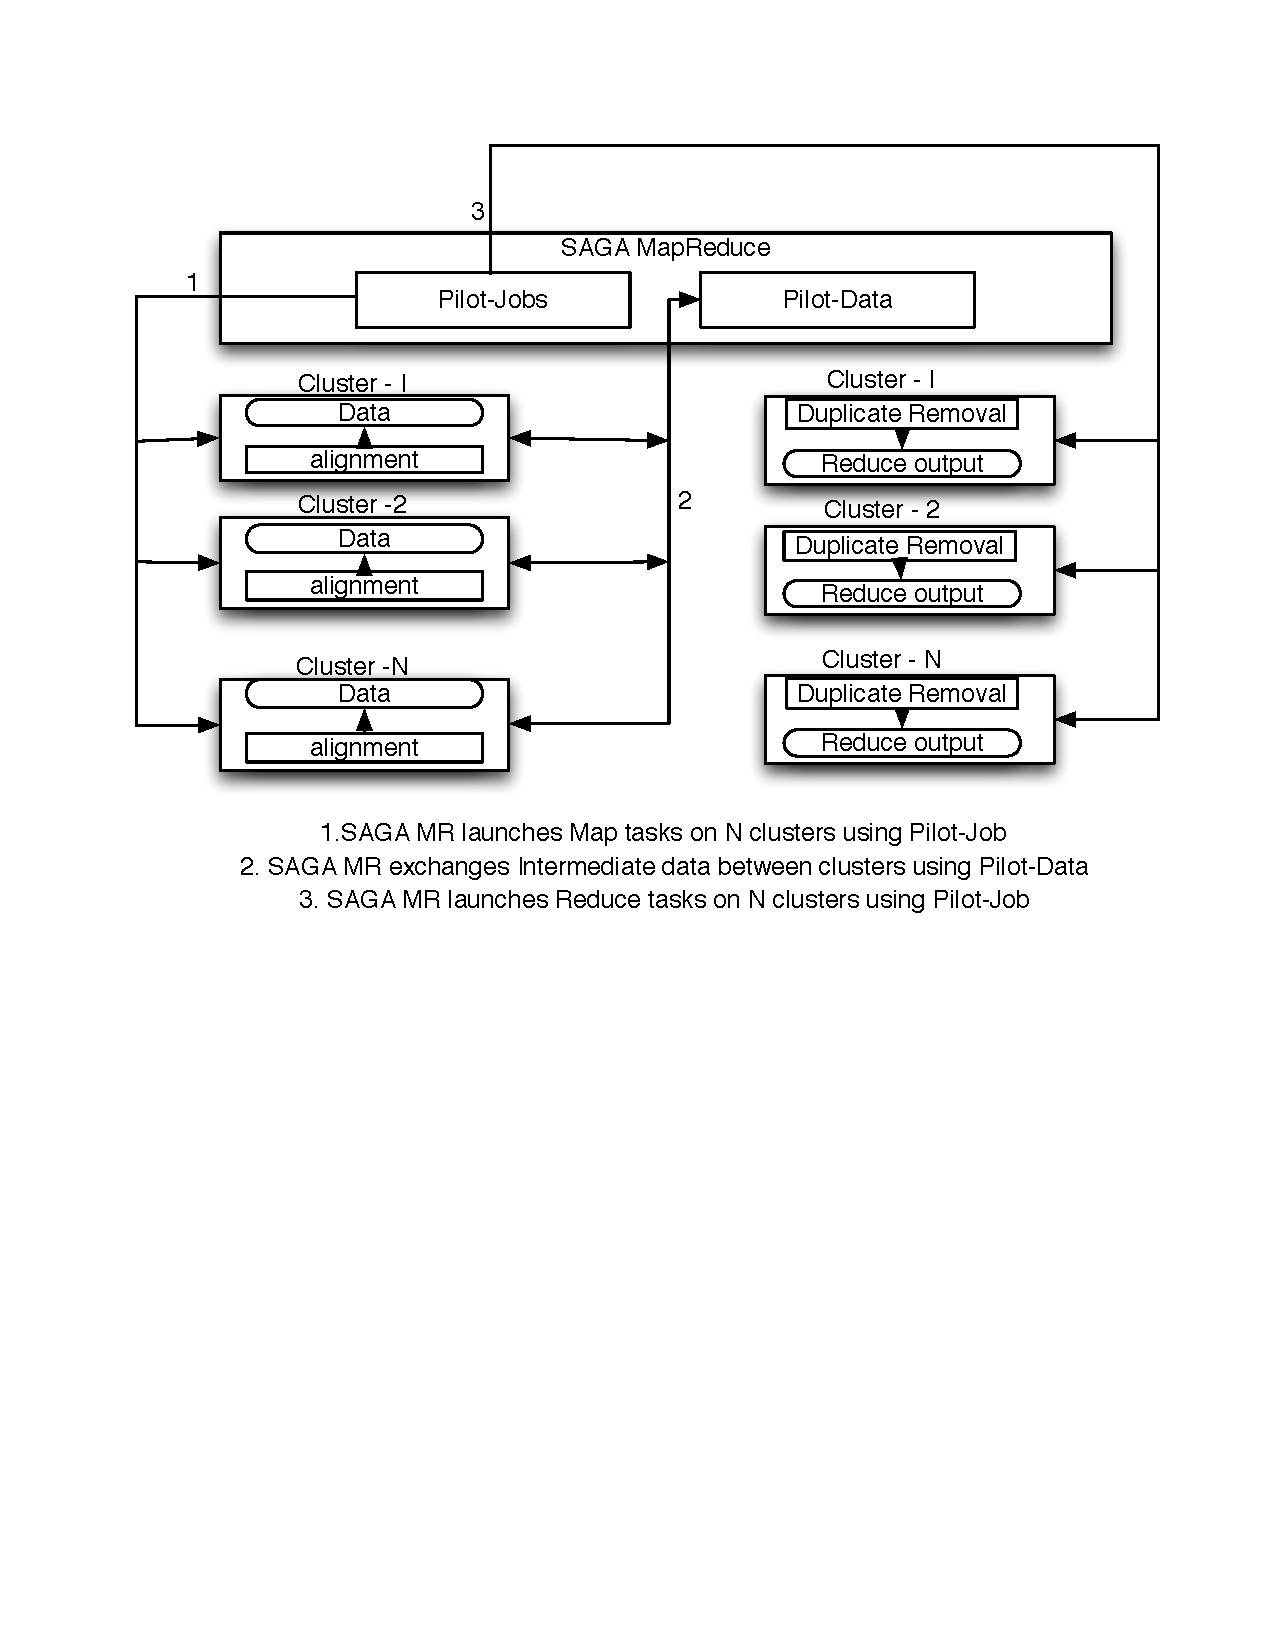
\includegraphics[scale=0.45]{figures/align-dup.pdf} 
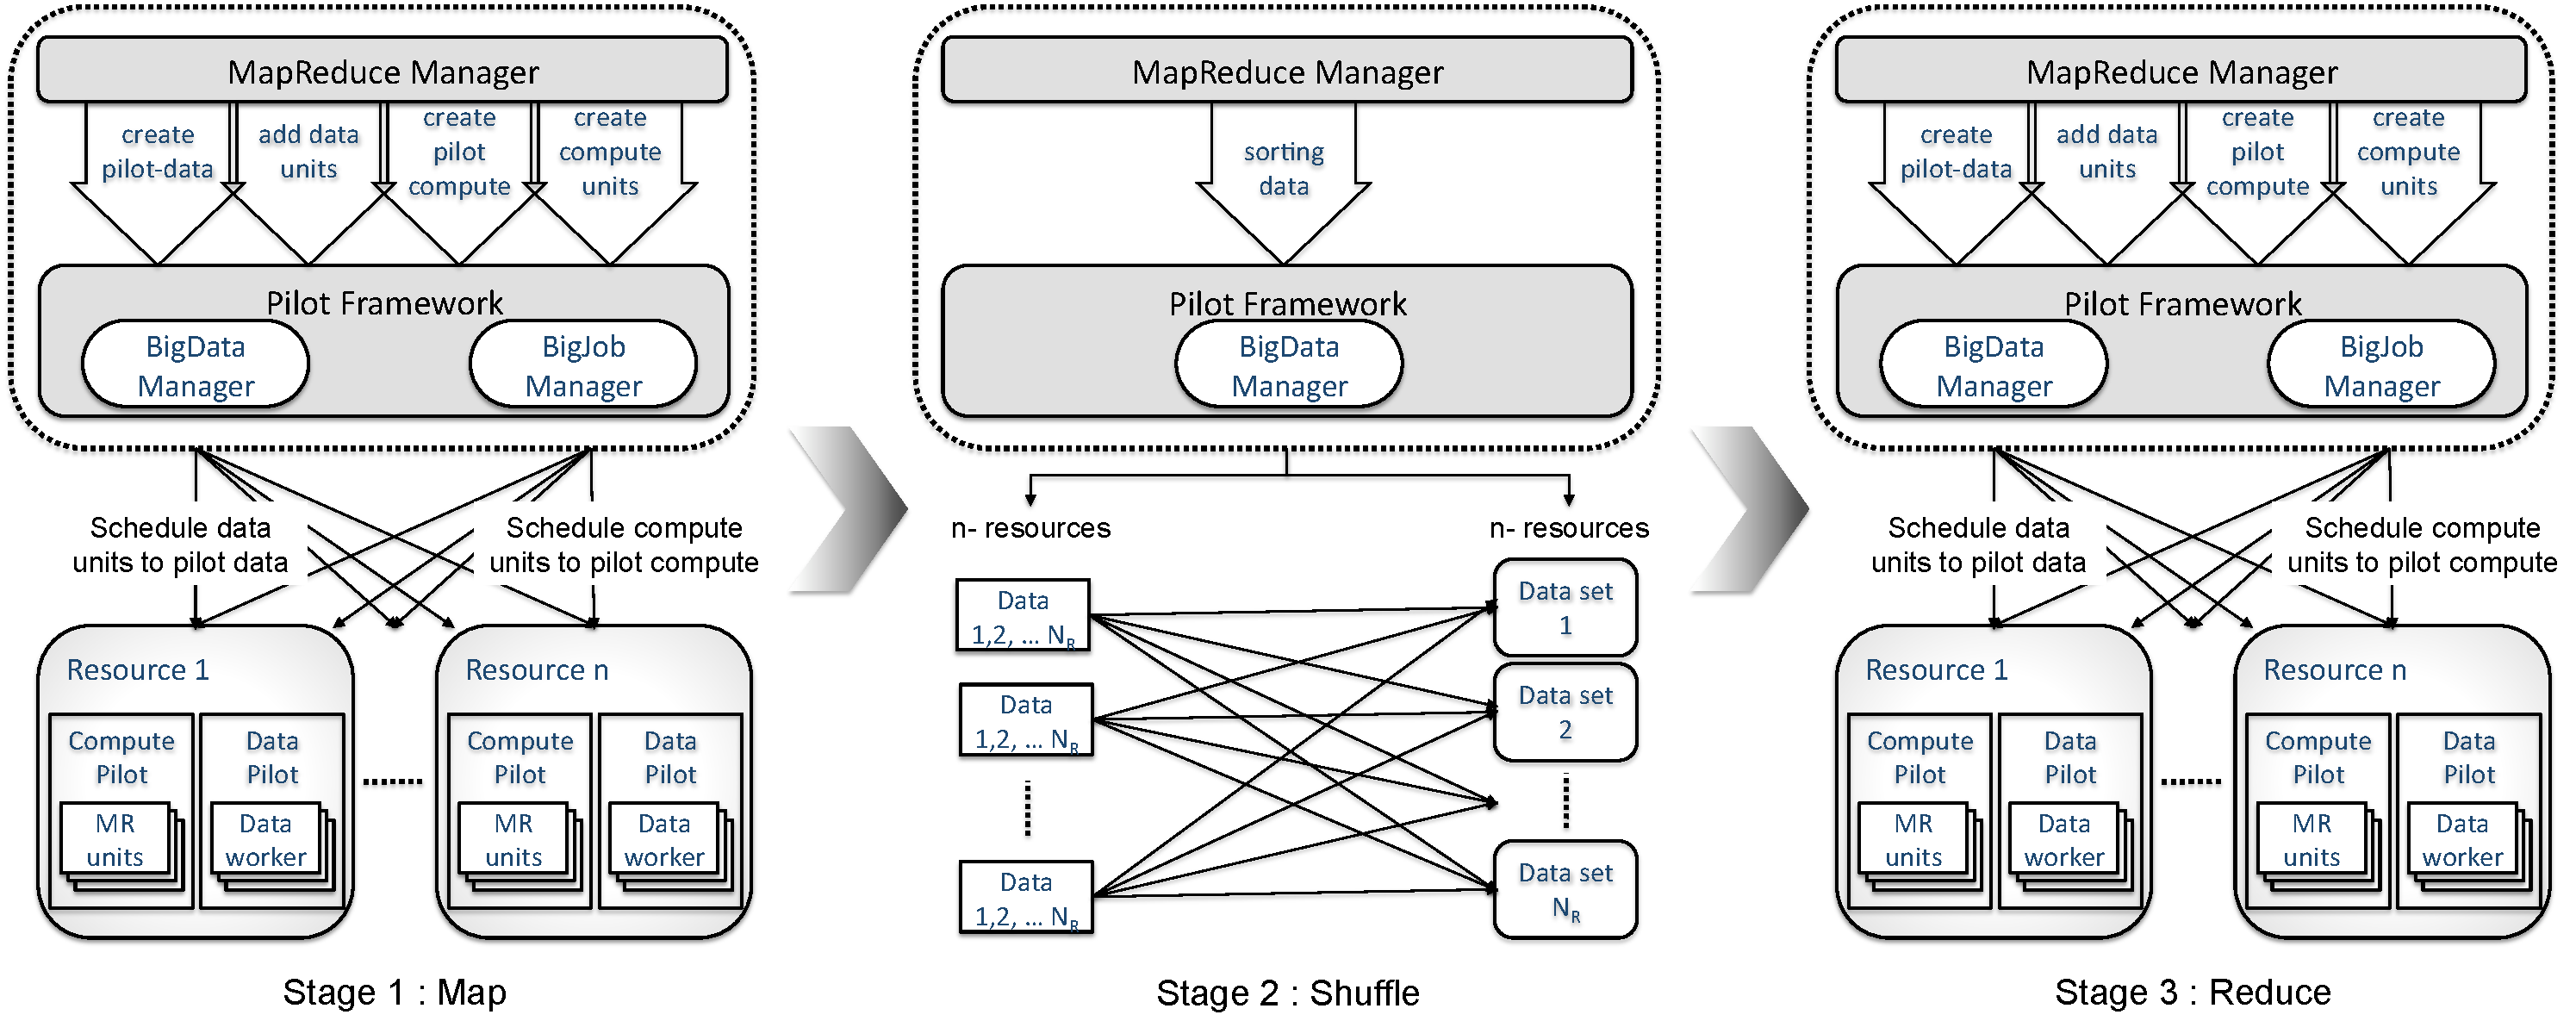
\includegraphics[scale=0.35]{figures/F1_1.pdf} 
\hfill{}
\caption{\small PMR architecture and the workflow for a MapReduce task}
  \label{fig:arch-pj-saga-mr} 
\end{figure*}
\end{center}

\jhanote{Merge: Since the paper about the MapReduce programming model
  from Google in 2004\cite{mapreduce-2004-dean} and the emergence of
  Hadoop, the model has drawn significant attention from various
  application domains as a general strategy for parallelization of
  processing a large data.  In recent years, the computational biology
  community, in particular focusing on data analytics and downstream
  analyses of high-throughput deep sequencing techniques such as NGS
  has found the potential of MapReduce-based approaches for dealing
  with unprecedented data produced from the novel
  platforms\cite{schatz-nature-biotech-2010}.  Not surprisingly, most
  of software tools using MapReduce for NGS data were developed with
  Hadoop environment and consequently with Cloud computing environment
  such as Amazon EC2.}

\section{Materials and Methods}\label{sec:materials_and_methods}
\subsection{NGS Data Sets and Target Analyses}
\subsubsection{Data Sets}

For this work, we used the paired-end sequence RNA-Seq data from the Flemington lab, which had originated from a Human Burkitt's lymphoma cell line\cite{erik_2010}.  The read length is 100 for both directions of paired-end data, and the total size of each data set is about 20.1 GB containing 70,927,422 reads.  For experiments of this work that use a varying size of sequencing data, we simply take the required amount of reads by partitioning the entire data.  For example, 2 GB input size implies 1 GB for one end and 1 GB for the other end data for dealing with paired-end data.  The file format of sequencing data is fasta and all manipulation of sequencing data was conducted by in-house python scripts and freely available tools such as samtools\cite{samtools}.  

\subsubsection{DNA Sequence Alignment}

The short reads alignment and the de-novo assembly are the required first steps in every pipeline software tool aiming biological discovery with sequencing data from NGS platforms.  Considering the fact that the de-novo assembly remains still challenging at this moment primarily arising from the complications with the short length of sequencing reads from NGS machines, in a practical sense, alignment or mapping is taken as the first task in most of cases.  In fact, for RNA-Seq data analysis, in particular with eukaryote genomes, the spliced aligner such as TopHat\cite{pepke2009} is needed. In this work, we consider the alternative strategy such that the non-spliced aligner is used and later splicing events are detected separately, justifying the use of non-spliced aligners such as BWA and Bowtie for the RNA-Seq data.  The reference genome used with these aligners is hg19.

\subsubsection{Other Data Analyses}

After alignment of sequenced reads onto the reference genome, a duplicate read removal step might be required because sample preparation processes before sequencing might contain artifacts stemming from high-throughtput read amplification; many duplicates introduced are not relevant to true biological conditions.  For characterizing our framework, we compare our results with the SEQAL tool of SEAL package since SEQAL aims to carry out the read alignment and duplicate removal.  SEQAL uses BWA for the alignment and for the duplicate removal, implements the same criteria as the Picard MarkDuplicates command\cite{seal2011,seal_2011_mapred}.  On the other hand, information about aligned reads are essential for many downstream analyses such as genome variation study, transcriptome analysis, and other various complex functional genomics and pathway analysis.  For example, Crossbow, the tool we investigated by the comparative experiments, aims to SNP finding along with aligned results\cite{langmead2009}.  Interestingly, Crossbow use the aligner, Bowtie, and thus our PMR-based tool is extended to implement Bowtie, in addition to BWA for the comparison with Crossbow.  Note that Bowtie is well-known for its efficiency in memory requirement and computation, but the current version doe not support gapped alignment whereas BWA does.

\subsection{Experiments: Motivation and Configuration}



A primary goal of this work is to use a PMR-based tool that is capable
of tasks combining the alignment and various downstream analysis for
genome structure studies, genotyping, transcriptome analysis,
DNA-protein interaction, and sequencing data process such as duplicate
read removal.  Our experiments primarily target the comparison of our
PMR-based approach with two other Hadoop-based approaches, SEQAL (tool
for alignment and duplicate removal) and Crossbow (tool for alignment
and SNP finding) that use slightly different Hadoop-based
approaches.(see Table~\ref{table:mr-comparison}).  Unlike such
Hadoop-based approaches to MapReduce, we show how a PMR supports
scalability across multiple distributed infrastructure including HPC
grids and Clouds.

The primary aim of the comparative experiments with SEQAL and Crossbow
are:

\begin{itemize}
\item Pros and cons of Hadoop-based approaches
\item Validate scalability via PMR and underscore the importance of the
  support of scale-across
\item Demonstrate PMR as a viable solution to (i) combine fine-grained
  and coarse-grained parallel approaches, (ii) support effective and
  efficient distributed data scenarios for NGS data analysis
\item Demonstrate importance of extensibility for multiple tool
  supports
\end{itemize}

\subsubsection{HPC Resources}
For this work, we used two Futuregrid systems, Sierra and Hotel.  More details on the specification of these machines can be found from the web page of Futuregrid\cite{futuregrid_url}.  In brief, two systems are multi-node clusters and equipped with the PBS job scheduler and Hadoop, implying that the systems are appropriate to test our PMR and to compare our results with Hadoop-based tools.

\subsubsection{MapReduce-based NGS Data Analytics using Pilot-based SAGA-MapReduce (PMR)}
The two combined steps such as alignment and duplicate removal or alignment and SNP finding are attractive targets for  parallelizing tasks by using MapReduce; the read alignment step is conducted as a Map phase and duplicate removal or SNP finding as a Reduce phase.  Note that a certain kind of combination for designing a MapReduce-based tool is immediately conceivable for other advanced downstream analyses such as transcript quantification or peak calling for other advanced NGS protocols.  The development for such tools will be announced in the future works.

The schematic workflow and architecture for running PMR is presented in Fig.~\ref{fig:arch-pj-saga-mr}.  As indicated, we need to configure computational tasks of the map phase and the reduce phase including the number of workers, available fine-grained parallelism options of software tools used for each phase, and configurations for Pilot Job (BigJob).  Note that we can choose many different combinations of these configurations (i.e. associated with parallel options with used software tools, and Pilot and MapReduce levels) for different strategies that tune the parallelism for a target analysis (in which map and reduce phases are decoupled, of course) differently by carefully considering fine-grained and coarse-grained parallelism levels.  Below, we describe more details on the parameters that we vary for a specific experiment.  Also, we consider the simple scenario with the Pilot configuration; we only create one PilotJob per each resource. For more details on the use of dynamic Pilot-based job execution, refer our previous publications\cite{dare-ecmls11,dare-tg11,repex_ptrsa}.    

As shown in Fig.~\ref{fig:arch-pj-saga-mr}, PMR implements a MapReduce task with the Pilot framework\cite{pmr2012} with the following workflow. 1.PMR launches Map tasks on N clusters using the Pilot framework. 2. After the Map stage, PMR exchanges Intermediate data between clusters using Pilot-Data of Pilot framework  3. Finally, PMR launches Reduce tasks on N clusters using Pilot framework.  Note that this unit of workflow can be extended to scenarios of hierarchical MR or distributed MR\cite{pmr2012}.  

\begin{center}
\begin{table*}[ht]
{\small
\hfill{}
\begin{tabular}{|l|l|c|c|c|c|c|c|}
\hline
  & \textbf{P-SAGA-MR}\cite{pmr2012} & \textbf{SEQAL}\cite{seal2011} & \textbf{Crossbow}\cite{langmead2009} & \textbf{CloudBurst}\cite{cloudburst} & \textbf{GATK}\cite{gatk} \\ \hline
%\cline{3-9}
 \hline 
Key Parallelism   & Pilot-based   &  Hadoop-based/  &  Hadoop   & Hadoop-based & MR-based Structured \\ 
Stretegy  & Distributed MR & MR  & Streaming  & MR & Programming  \\
& & (Pydoop) &  & & Framework  \\ \hline
  
Hadoop & No & Yes & Yes\footnote[1] & Yes & No \\ 
Requirement  & & & &  &\\ \hline  
    
Multiple  Cluster & Yes  & Limited   & Limited  & Limited  & Limited \\
Support &  & by Hadoop &  by Hadoop & by Hadoop  & by JVM   \\ \hline

Multiple Node & Support & Not allowed  & Not allowed  & Not allowed & Not  \\
Task Supprt &  & by Hadoop & by Hadoop & by Hadoop & Easy  \\ \hline
Distributed Job and  & Advert Service  & Hadoop/HDFS & Hadoop/HDFS & Hadoop/HDFS & Java \\ 
Data Coordination &(SAGA) &  & & & Framework\\ \hline


Primary Aligner &  BWA, Bowtie,  &  BWA & Bowtie & RMAP &  BWA \\
& and Others (coming) &  &  &  &  \\ \hline
Multiple Aligner  & Straightforward & Not Straight- & Possible & Not Straight-  & Straight-  \\ 
Support &  & forward &   & forward  & forward \\\hline
Primary Tasks & Alignment/Duplicate  & Alignment/ & Alignment/ & Alignment &Various\\
  &  Removal & Duplicate & SNP Discovery & & NGS Data  \\  
           & (and Extensible &  Removal & &  & \& Downstream  \\
           & for RNA-Seq) & & &  & Analysis \\ \hline  
Extensibility for   &  High  & Medium &  Low & Low & High      \\
Multiple Tools  &      &  &  &  &   \\ \hline

\hline
\end{tabular}}
\hfill{}
\caption{Feature comparison of PMR with other tools for NGS data analysis that primarily provide a parallelism support using the MapReduce framework.  $^{1}${The feature of Crossbow that can run with a desktop environment without Hadoop is not considered in the scope of this work due to the lack of scalability support.} }
 \label{table:mr-comparison}
\end{table*}
\end{center}

\subsubsection{Comparative Experiments with two Hadoop-based tools, SEQAL and Crossbow}
Among the software tools compared in ~\ref{table:mr-comparison}, we chose SEQAL of the SEAL package and Crossbow for the comparison.  Note that these two tools along with other tools such as Cloudburst and GATK are different from each other with respect to the usage mode of MapReduce and the design strategies behind each tool for parallelism, in particular, aiming NGS data processing and management as summarized in Table~\ref{table:mr-comparison}.  Importantly, SEQAL and Crossbow are Hadoop-based tools but differ in that the former is designed conventionally with implementing Map and Reduce functions whereas the latter uses Hadoop-streaming.  In the case of Crossbow, the overall analysis is taken with 4 steps.  Each step is an independent Hadoop-streaming task.  The first step is for pre-processing and the last one is for post-processing. The second one is for the alignment and the third one is for SNP finding, which uses slightly modified Bowtie and SOAPsnp.  

For the two applications, SEQAL and Crossbow, Hadoop version 0.20.2 was used with the two FutureGrid machines.  For SEQAL experiment, SEAL version 0.2.3 was used and for Crossbow experiments, we used version 1.1.2 that contains bowtie version 0.12.7 and soapsnp version 1.02.  For SEQAL and Crossbow experiment, the replication factor for Hadoop configuration is set  to 2.  If not specified, all options for aligners and external tools as well as SEQAL and Crossbow setting are default as suggested.  For example, SEQAL does not support the multi-threading option of BWA, whereas Crossbow sets up the default option for Bowtie, "--mm" to support running many concurrent Bowtie processes on a node while sharing the memory index to avoid memory overhead effectively.  

The input file format for SEQAL is prq format.  To convert a fasta format sequence file to this format, we use SEAL, a software tool containing SEQAL as a part that has a file conversion capacity between qseq/fastq and prq format.  

\begin{table}
\small
 \begin{tabular}{|c|c|c|c|c|c|} 
 \hline 

Case & \# of  & \# of &  \# of & \# of & \# of  \\
E($N_{node}$,$N_W$,  & Nodes & Worker   & Mapp- & Reduc- & available  \\
$N_M$, $N_R$,  & &  & ers & ers & cores per\\
$S_I$ (GB)) & ($N_{node})$& ($N_W$) & ($N_M) $ & ($N_R$) & Worker \\
 \hline
E(4, 4, 32, 8, 8) &4 &  4 & 32  & 8 & 8 \\
E(4, 8, 32, 8, 8) & 4 & 8 & 32 & 8 & 4 \\
E (8, 8, 32, 8, 8) & 8 & 8 & 32 & 8 & 8 \\ 
 \hline
 \end{tabular}

 \caption{Description of experimental cases examined in this paper for understanding scalability, impact of parallelism strategy, and performance comparison.  A experiment will be described with the five parameters in E($N_{node}$,$N_W$,$N_M$, $N_R$,$S_I$).  Three examples are illustrated in this table.  Note that all nodes for this study have 8 cores and the number of cores per Worker is determined by the total number of cores divided by the number of Workers in a node.}
    \label{table:exp-description} 
\end{table}

In the case of Hadoop-based MapReduce tools, we set the number of workers per a node ($N_{W/node}$), the number of mappers ($N_M$) and the number of reducers ($N_R$) via Hadoop configuration or tool configuration.  These number should be carefully chosen along with the parameters for the size of resource, i.e., the number of nodes ($N_{node}$) and the given number of cores in a node.  For example, the memory size of a node wold limit a possible choice for $N_{W/node}$ since such multiple workers in a node might need more memories than the total memory of the node and consequently fail to run.  Importantly, note that such parameters dictate the parallelism of a target task with MapReduce configuration as well as fine-grained parallelism that might be implemented in tasks for Map or Reduce phases.  For the input data partitioning, if not specified differently, the default chunk size of 128MB was used, which corresponds to nearly 292,763 reads.  For example, the size of 2 GB input is broken into 16 files (8 files for each end data) and importantly results in 8 Map phase tasks.  Note that in the case of SEQAL that uses the different format, the chunking process generates the same amount of reads per file.  This chunk size is directly related to the number of Mappers $N_M$ for the alignment task since  $N_M$ is determined as the ratio of the size of input($S_I$) over this chunk.   For the relation between parameters used for the experimental set-up, see the examples in Table\ref{table:exp-description}. 
%$N_{W_{node}}$
%The configuration , we set the number of nodes as 4, and the maximum map and reduce tasks is set to be 2.  We found that if the number of tasks is set to be more than 2, the issue with memory size occurred.  \pmnote{refer to reference paper}  Thus, total 8 workers were used.

PMR set-up is as follows.  Similar to the Hadoop-based MapReduce tools, the configuration requires to set $N_{node}$, $N_W$, and the size of BigJobs that is a task container in our Pilot framework\cite{pmr2012,saga_bigjob_condor_cloud,pstar11}.  Note that $N_W$ has no limitation with the size of a node since multiple-node worker is possible when a tool executed by a work supports multi-node parallel implementation such as MPI.  Thus, with PMR, we set $N_W$, instead $N_{W/node}$.  Since BWA and Bowtie have an option for multi-threading, with PMR, we can provide the configuration for the option as ON or OFF to understand the impact of such fine-grained parallelism along with coarse-grained parallelism with the MapReduce framework.  Note that SEQAL and Crossbow turn off this option as default.  Also, multiple clusters can be used for MapReduce. For example, the half of workers are assigned with Hotel and the other half in Sierra.  For a single system set up, like the two Hadoop-based MapReduce tools, all workers are now running in the system.  

Data management is an important component for any tools processing distributed data with parallel strategies and the efficiency of data transfer should be considered when a MapReduce-based tool is assessed.  Whereas Hadoop-based approaches relies upon HDFS and TCP/IP-based communication between data nodes, PMR uses SAGA Advert coordination among workers via Pilot framework (see Fig.~\ref{fig:arch-pj-saga-mr}).  PMR, indeed, is flexible and extensible for scaling across multiple clusters without the global file system support.  
 
%   \pmnote{chunksize = number of lines of fastq file ( number of sequences (292763 * 4 ) since in fastq each sequence is of 4 lines..
%tts = max( map on Sierra, map on Hotel)+max( time tansfer from Sierra to Hotel, time transfer from Hotel to Sierra)+max(reduce on Sierra, reduce on Hotel)..
%Graph : x axis- (2,4,8 input sizes) with chunk size 292763 sequences, number of workers=8, reduces=8.
%experiments repeated thrice.. }
 
For the experiments with PMR using distributed resources, we assume
that all input and required data are stored initially on a single
cluster to process and measure the time for distributing data.



\section{Results}\label{sec:results}

\subsection{PMR for NGS data analysis : Reads Alignment and Duplicate
  Removal}

The computation of read alignment and duplicate removal represents an
interesting and simple category of computational tasks among NGS data
analysis that could be benefitted by employing the MapReduce
programming model.  We implement such a MapReduce task with PMR.  The
main findings with this analysis are as follows.  First, as shown in
Fig.~\ref{fig:read-size}, the scalability is critically required as
the input data size increases.  Not surprisingly, the results shown in
Fig~\ref{fig:scale-p-saga-mr} suggests that the parallel strategy with
MapReduce could be a viable solution for increasingly demanding large
data sets.

 \begin{figure}
 \centering
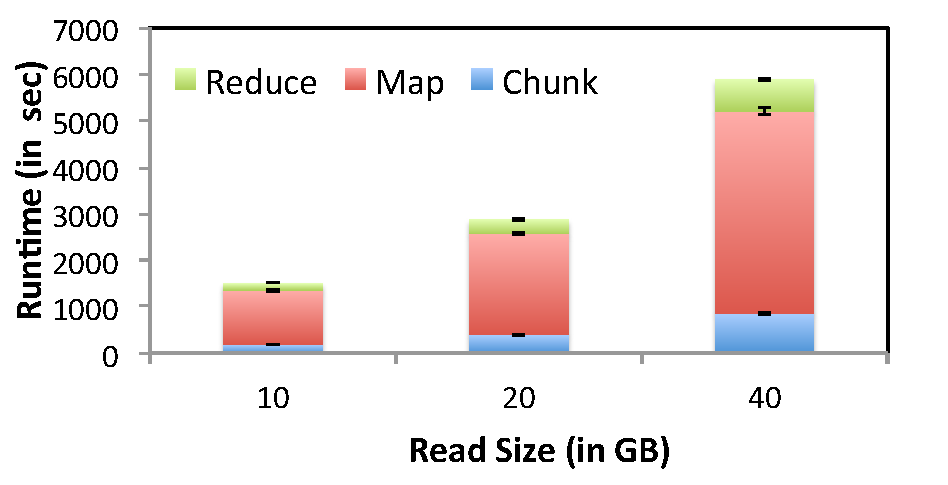
\includegraphics[scale=0.50]{figures/pj-smr-tts.pdf} 
\caption{\small Need of a scalable solution with increment of data volume.  Read size dependent time-to-solution is measured for MapReduce tasks of read alignment and duplicate removal.  The number of nodes for this experiment,$N_{node}$ is 16, the number of Workers, $N_W$ is 32, and the chunk size is set to contain 62500 reads.  The number of Reducers is set to 8. BWA is used for read alignment.}
  \label{fig:read-size} 
\end{figure}


The good scalability with PMR shown in Fig~\ref{fig:scale-p-saga-mr}, as a matter of fact, appears to be helped by the characteristic nature of the target computational tasks.  The Map phase, the read alignment is a single dominant step for the overall time-to-solution, and the read alignment task is the most prominent example among a variety of NGS data analysis tasks that is suitable for data parallelization as well as task parallelization.  Note that the Reduce phase task, duplicate removal is also easy for parallelization primarily due to the fact that to remove the duplicates needs only the local information, i.e. a single key or a small number of keys from the Map phase results.  Despite of the simple nature, read alignment and duplicate removal does provide an understanding of challenges for MapReduce-based approaches for NGS data analytics.  For example, unlike the well-know word count problem, the Map phase produces high volume of data size, indicating the low-aggregation problem, compared to the high-aggregation problem of the word counting\cite{weissman-mr-11}.  Indeed, the data management along with this feature should be considered carefully as indicated in Fig.~\ref{fig:read-size} with the 40 GB case that shows a significant portion of the processing time for chunking data.  Note that 40 GB is the entire data set from the RNA-Seq experiment of interest.  Nonetheless, we note that the data management between the Map phase and the Reduce phase is reasonably handled by the Pilot framework for a single cluster or even a case for utilizing a couple of clusters as presented later.


\begin{figure}
 \centering
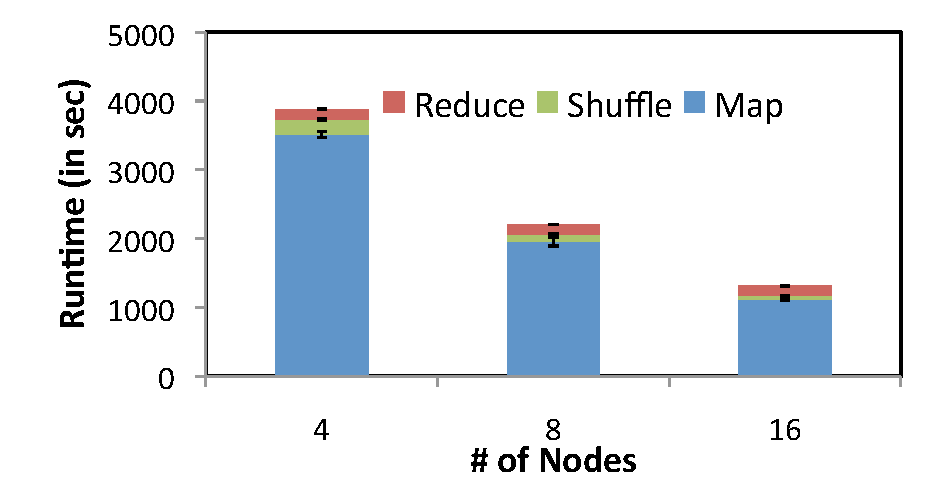
\includegraphics[scale=0.50]{figures/pj-smr-scale.pdf}
\caption{\small PMR scalability of a MapReduce-based computation for read alignment and duplicate removal.  The number of Workers per node, $N_{W/node}$ is set to 2.   The input read file is 10GB, the number of Reducers is set to 8, The number of reads in a chunk is 625000. BWA is used for read alignment}
\alnote{I thought we don't include PMR only data}
  \label{fig:scale-p-saga-mr} 
\end{figure}


\subsection{Comparison to Hadoop-based SEQAL and Crossbow}
\subsubsection{Closely Related Works}
Compared to other areas, the computational biology community, specifically focusing on NGS data analysis, joined later for the use of MapReduce\cite{cloudburst}.  Nonetheless, there have been active works resulting in the programs listed in Table~\ref{table:mr-comparison}.  In brief, Cloudburst was one of the first generation tools in this field and  demonstrated the significant potential of the MapReduce model for NGS data analysis.  After Cloudburst, Crossbow was developed by focusing on better scalability using Hadoop streaming.  Compared to the two Hadoop-based tools, GATK was introduced to address the general parallel execution pattern across many NGS data analytics.  Recently, the SEAL package was announced in which SEQAL is a utility for the alignment and duplicate removal.   

In spite of the commonality that MapReduce is the core programming model for the tools, they differ in several aspects depending upon the need of Hadoop, the way to utilize Hadoop, the level of flexibility for the extension of tools for alternative tasks or the multiple tool support for different aligners, for example, and whether the multiple cluster support is possible.

Interestingly, the cross-domain support over multiple clusters with the MapRedue framework, specifically via so called hierarchical MapReduce, was recently suggested for the AutodDock tool.  We note that this docking application belongs, in contrast to our applications that are mostly loosely-coupled, to pleasingly parallel and thus faces a different bur simpler type of challenges, compared to ours\cite{ecmls11-mr-autodock}.

To demonstrate the distinctive strategies and features of PMR-based tools, we compare the performance with SEQAL and Crossbow in the followings.  

\begin{figure}
 \centering
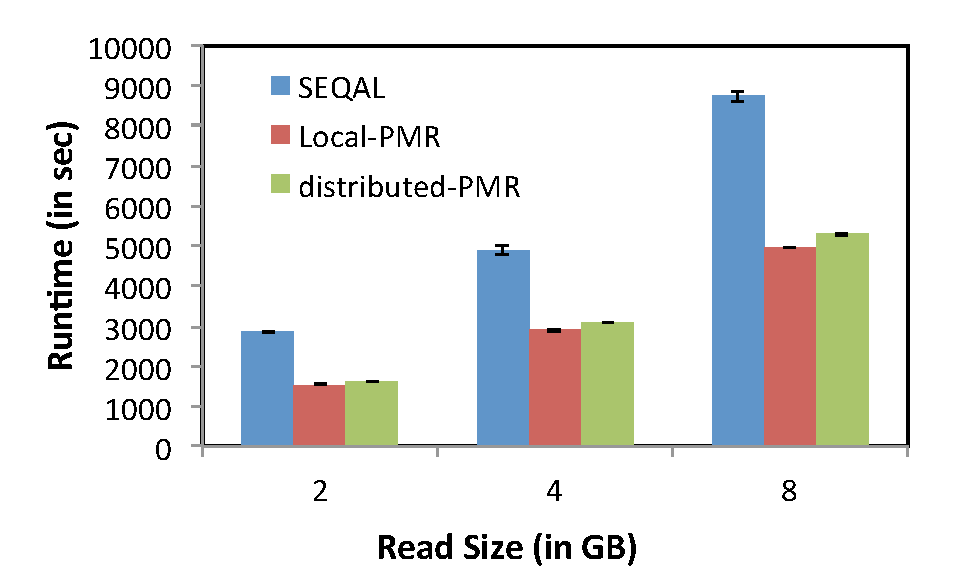
\includegraphics[scale=0.50]{figures/seqalvslocalpmr.pdf}
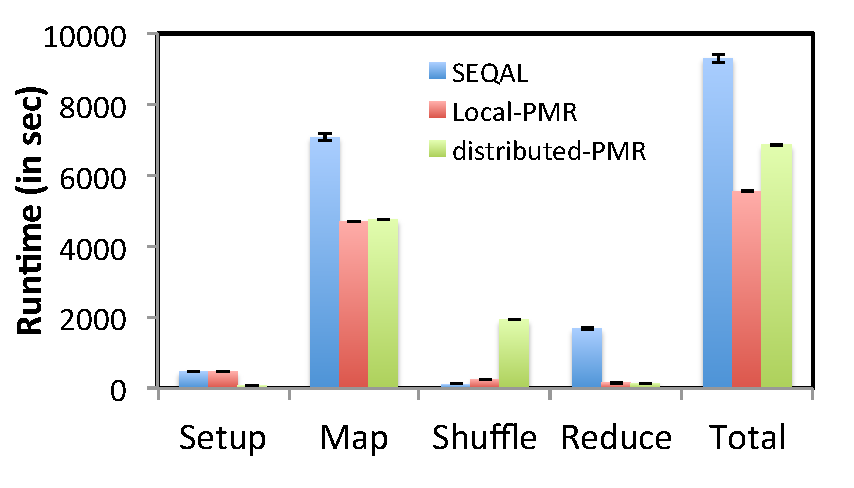
\includegraphics[scale=0.52]{figures/8GB_phasewisetimes.pdf}

\caption{\small Comparison of the total time-to-solution for a MapReduce-based computation of alignment and duplicate read removal (upper).  Dissected elapsed times for each step of the results with 8 GB (lower). Hadoop-based SEQAL is compared to Local-PMR vs. distributed-PMR.  BWA is the aligner for the map phase.  The size of input is 8 GB.  For this experiment, the number of Nodes, $N_{node}$ is 4, the number of Workers, $N_W$ is 8, the number of Reducers, $N_R$ is 8, and the number of reads in each chunk is 292,763. For the distributed-PMR, two machines of FutureGrid, Sierra and Hotel were used, whereas Sierra was used for other cases.}
\alnote{same analysis in in MR paper}
  \label{fig:comp_with_seqal_1} 
\end{figure}

\subsubsection{Performance Comparison}
In Fig.~\ref{fig:comp_with_seqal_1}, we compared directly the time-to-solution between SEQAL and two scenarios with PMR, one with a single cluster and the other with two clusters.  In Fig.~\ref{fig:comp_with_seqal_2}, also how each step contributes for the total runtime is presented with the case of 8 GB input.  

Notably, SEQAL takes more time on the overall run time, and the most
contributing cause for benchmark difference comes from the Map phase.
We contribute this result with the situation of the Hadoop
configuration with the FutureGrid systems.  The tmp directory accessed
by workers of each node is configured by Hadoop, but the size of a tmp
directory is limited with the fast and local attached disk space and
thus a remote file system is configured as the tmp data directory.
This situation is likely to enforce most of users, a non-expert on
Hadoop system, and results in the performance loss with File I/O.  The
similar observation was also indicated with the comparison of
Crossbow.

Another important aspect which can be inferred from results shown in
Fig.~\ref{fig:comp_with_seqal_1} is that whereas SEQAL is limited by a
single cluster with Hadoop, PMR can be easily scale-across over
multiple clusters. The distributed-PMR, which uses the two cluster
systems, Hotel and Sierra, is indeed performing well against the
local-PMR in spite of the low network connectivity between two
clusters compared to a intra-cluster network connection.  The overhead
arising from the connection between two clusters is indicated in
Fig.~\ref{fig:comp_with_seqal_1}(lower) by showing the longer time for
shuffling in the case of "distributed-PMR".

Note that the direct comparison of the Reduce phase is not straightforward due to the potentially different implementation between SEQAL and ours in spite of the fact that we used the same criteria of the duplicate removal of SEQAL\cite{seal_2011_mapred}.  In any event, unlike the Reduce phase, the Map phase of SEQAL and our PMR tool are almost comparable since the same aligner, BWA is used and all parameters (see Table~\ref{table:exp-description}) for configuring a MapReduce task are same in the comparison.   



\begin{figure} 
 \centering
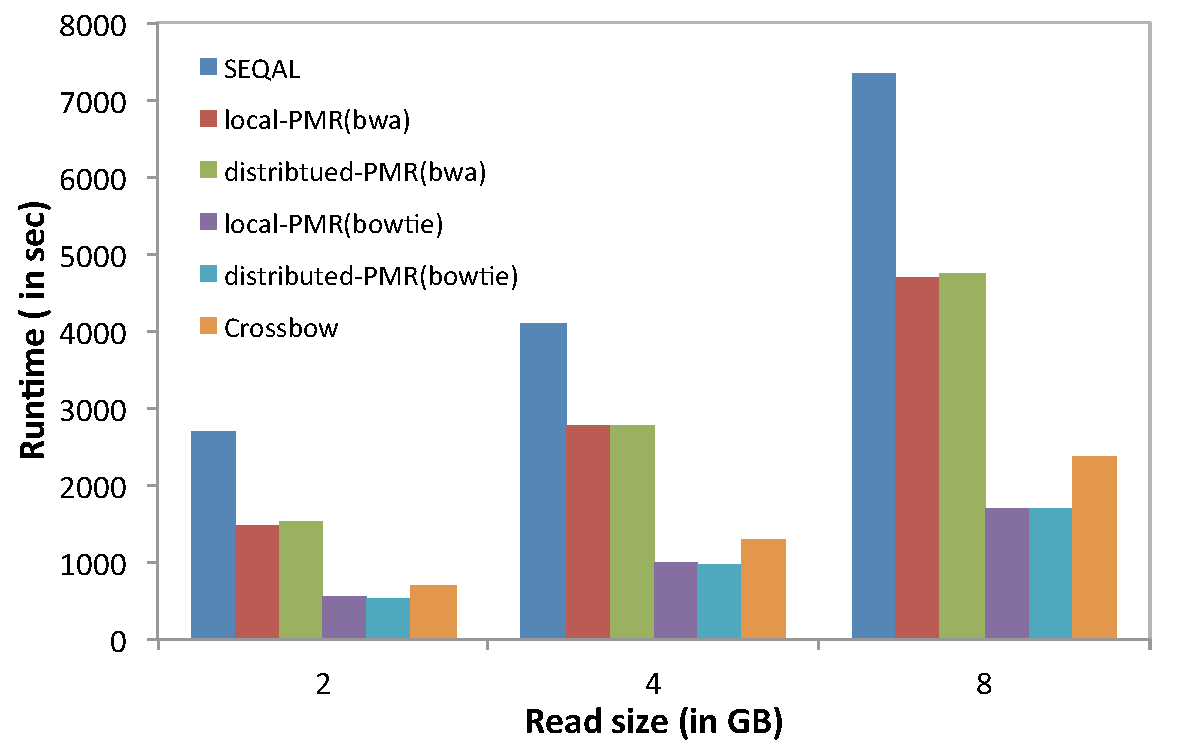
\includegraphics[scale=0.40]{figures/map_comp.pdf}
\caption{\small  Map phase comparison.  The runtimes for the Map phase of SEQAL, Local-PMR(BWA), distributed-PMR(BWA), Local-PMR(Bowtie), distributed-PMR(Bowtie), and Crossbow(Bowtie) are compared.  The aligner used for each case is indicated in a parenthesis.  For this experiment, the number of nodes, $N_{node}$ is 4, the number of Workers, $N_W$ is 8, and the number of reads in each chunk is 292,763.  For the distributed-PMR, two machines of FutureGrid, Sierra and Hotel were used, whereas Sierra was used for other cases.}
  \label{fig:tool_comp} 
\end{figure}

%number of nodes=4, number of workers/node=2,reduces=8, number of reads/chunk=292763; ********DMR provides scale-across********** as two machines Sierra and Hotel are used.

Another Hadoop-based tool, Crossbow, uses Bowtie as a aligner and
utilizes Hadoop-Streaming\cite{hadoop-url}.  We summarize the result
of measuring the times of alignment step calculations and present in
Fig.~\ref{fig:tool_comp}.  The tendency shown with the comparison of
SEQAL to PMR is also observed with the comparison with Crossbow; the
longer runtime with the Hadoop-Streaming-based tool regardless of the
use of a different aligner, Bowtie.  It is well-known that Bowtie is
extremely efficient in computation of alignment and the results found,
correspondingly, less time-to-solution with the aligner.


%As the number of input sequences increased the time to solution also increased linearly for both SEQAL and local-PMR. 
%The time to solution decreased by an average of 43.39\% with 95\% confidence interval of 3.03\%. The Map phase of Local-PMR is on an average of 64\% of Map phase of SEQAL application, and is reduced by an average of 35.7\%
%The reduce phase is very less compared to seqal applicaiton because there is not sort involved in reduce phase.
%\pmnote{( why is that?? i dont see any reason to have a sort before reduce starts)) we do sort intermediate data before shuffled.}
%The reduce phase is average of 8.85\% of reduce phase of seqal  ( it involves sort )
%
%\pmnote{how to explain performance of PMR ??}..One of the performance bottlneck for PMR is coordination system used... we used redis as coordination system... which is proved best ,when compared to other coordination systems{Pstar reference}. I think we can compare the results.. but cant say why SEQAL performed better.. since, it needs understanding of how SEQAL actually works.

\subsubsection{Scale-across, Extensibility, and Parallelism Support}
The scale-across over multiple clusters and the ease of extensibility are two important advantages with the PMR as indicated with the benchmarking results.  The ease of extensibility is particularly demonstrated with two aligners, BWA and Bowtie support.  One of the important reasons why multiple aligners are needed is because of the difficulty of validation of an aligner used.  It is well studied that each aligner implements different strategies to deal with the requirement of computational loads, memory usage, and sensitivity associated with decision on algorithms and computational implementations of indexing, search, and match tasks\cite{mapping-survey}   Indeed, the decision of an aligner affects not only alignment results but also scientific discovery with downstream analysis aiming genome variation study, transcriptome analysis, and DAN-protein interactions. Therefore, it is not overstated to emphasize the importance of supporting multiple tools as well as providing an effective means for implementing such tools within a reasonably short development period for infrastructure of NGS data. 


\begin{figure} 
 \centering
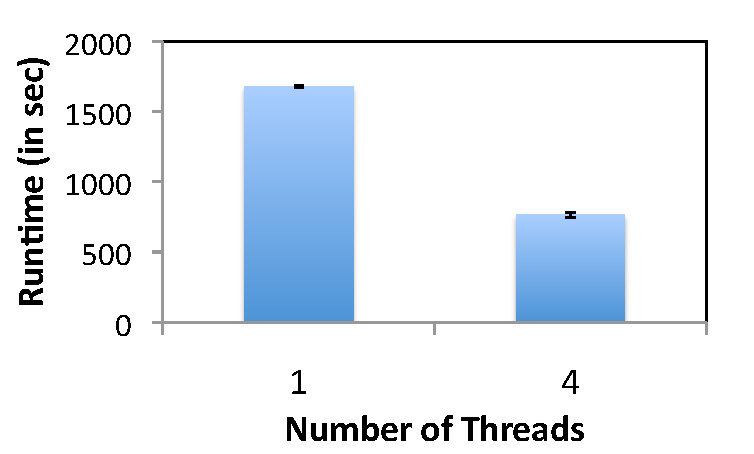
\includegraphics[scale=0.50]{figures/8GB_4nodes_8w_threadcomp.pdf}
\caption{\small  The performance role of multi-threading support option is indicated.  $N_W$=8, $N_{node}$=4, and input data size is 8 GB.}
  \label{fig:mulit-parallel} 
\end{figure}

Last but not the least, PMR has an advantage to manage multiple levels of parallelisms and optimize them for the efficient execution to lower time-to-solutions.  BWA and Bowtie have a fine-grained parallelism option with the multi-threading support option.   In Fig. \ref{fig:mulit-parallel}, we showed how such an option could affect on the performance.  
Even though it is feasible for other tools such as SEQAL or Crossbow to handle such options, our approach to combine the Pilot framework and the MapReduce framework is easily capable of utilizing the fine-grained parallelism along with the parallelism provided by MapReduce.  One important discussion in this line of direction is that our PMR is also able to optimize the multiple levels of parallelism when a standalone executable run by MapReduce is an MPI application.  Previously, we reported the usefulness of our Pilot-Job framework for such a situation\cite{repex_ptrsa}.  Note that it is not straightforward or impossible for Hadoop-based approaches to deal with multi-node applications.


\section{Discussion}\label{sec:discussions}
\textit{Computational Challenges for NGS data analysis, processing, and downstream analysis}

In the last several years, every area of biology and biomedical fields
has witnessed a paradigm change with DNA sequencing data generated by
NGS
platforms\cite{metzker2010,1000genome,wang2009-natrevgen,alex2009,mcpherson2009}.
Most importantly, these high-throughput technologies were able to
provide the thorough information about an entire genome or
statistically meaningful number of genomes of same species or related
ones with enormously affordable cost, resulting in an influx of
unprecedented amount of data.  While there have been algorithmic
advances and a plethora of new software tools particularly leveraged
by user-friendly interface via web-based tools, GUI tools, or computing environments \cite{galaxy}, the holistic infrastructure
development is lagging behind the community-wise demand.  One of
important conner stones for such development is to support scalable
computational tasks or distributed data management.  MapReduce is a
widely employed programming model for parallelization of a large data
process, and as reported by others with the tools listed in
Table~\ref{table:mr-comparison}, we observed that PMR based on
MapReduce provided the efficient methods for dealing with the required
scalability of NGS data analysis which comprises short reads alignment
and other following analysis such as duplicate removal and SNP
finding.

%First, as shown in  Fig.~\ref{fig:read-size} and Fig.~\ref{fig:scale-p-saga-mr}. the Map phase, read alignment, takes significantly more time than the task with the %Reduce phase, duplicate removal or other steps such as chunking input dta.  Secondly, the Reduce phase task, like the Map phase task, i.e. read alignment, additive.  %Here, the term additive means $f(X + Y) = f(X) + f(Y)$ where $X$ and $Y$ are input variables and $f$ represents the Map or the Reduce function.  On the contrary, SNP f%inding or other advanced NGS analysis are not in this type of analysis.   


\textit{PMR, a viable solution for scale-across and extensible framework for NGS data analytics}

PMR is a unique framework combining the MapReduce framework and the Pilot-based framework for distributed task and data management\cite{pmr2012}.  Considering the usefulness of data parallelization and processing for sizable NGS data and its analysis that might need the utilization of distributed compute resources and data storage, this combination of two frameworks implemented in PMR is the key aspect that positions PMR as a viable framework for a diverse set of NGS data analytics and downstream analyses.  In addition, the Pilot framework of PMR provides a runtime environment with which minimally modified standalone target tools are executed in multiple network-connected infrastructures and the overall workflow can be dynamically optimized by exploiting multiple levels of parallelism strategies as shown with our results.    Furthermore, as indicated in the results to show the support of multiple tools (BWA and Bowtie for alignment), the design strategy behind PMR is to allow an effective development cycle for further extensions of of existing implementation with other complementary tools or a flexible pipeline development.  In fact, our primary goal behind this work is to develop an integrative pipeline service for RNA-Seq data, and our development presented in this work is indicative of preliminary progresses toward such a goal. 

\textit{PMR vs. Hadoop-based MapReduce tools}

The open source Hadoop provides an ideal environment for the tools
based on the MapReduce programming model.  Perhaps, the ease of
installation with commodity hardware and the robust stability with
fault-resilency and easy scalability could propel a wide acceptance of
Hadoop.  Nonetheless, Hadoop-based approaches find many huddles when
the scalability across multiple clusters\cite{weissman-mr-11}, the
execution of applications across multi-nodes such as one using MPI,
and the solutions resolving limitations imposed by a current Hadoop
implementation need to be addressed.  For example, due to the issue of
scalability with Hadoop for a large scale problem, already discussions
and suggestions for the next-generation Hadoop have been circulated in
the community\cite{ng-hadoop-url}.  Indeed, as evidenced with the
comparison of our PMR-based read alignment and a following analysis
with two Hadoop-based tools, Crossbow and SEAQL, distinctive
advantages of our PMR-based implementation are clearly demonstrated
for such issues.

%It was reported that the overall performance of Hadoop-based MapReduce is determined by the unknown network performance and the connectivity between the data storage and the compute which are determined by characteristics of the cluster Hadoop is installed.  The tight coupling between the MapReduce applications with underlying Hadoop causes unnecessary complexity when the optimization or the design of parallel execution is required.  Secondly, it is not trivial to scale across different clusters.  Many issues on the connectivity between two separate clusters including firewalls, different security policies, and potentially different administration structure are making difficult to extend Hadoop with other cluster systems.  Thirdly, it is a still ongoing concern that Hadoop's current implementation has obstacles from the scalability issue with the design with Namenode and Job tracker.   The open source Hadoop is implemented with a job and task tracker: the job tracker is the central manager that dispatches map and reduce tasks to the nodes(nodes could be from multiple clusters) of the Hadoop cluster. On each node the task tracker is responsible for executing the respective tasks. The main limitation of this architecture is the fact that it intermixes both cluster resource management and application-level task managements. Thus, it is e.g. not easily possible to integrate Hadoop with another resource management tool, e.g. PBS or Torque. Also, the job tracker represents a single point of failure and scalability bottleneck. Another limitation is the latencies between machines should not be so big as HDFS uses Avro - an RPC-style protocol for communications.
%
%Collectively, PMR has edges in terms of flexibility and non-Hadoop-based architecture


\textit{DARE and beyond}

PMR-based NGS tools, implemented and scrutinized in this work, were developed in conjunction with our development of the runtime environment for dynamic applications, Dynamic Application Runtime Environment (DARE)\cite{dare-tg11,dare-ecmls11}.  DARE is our strategically important component for the development of Science Gateway for NGS data analytics and downstream analysis.  Under the design strategy of DARE-based gateways, PMR-based tools were conceived to be a main category of supporting execution patterns for parallel and distributed task and data management.  




\section*{Acknowledgement}

The project described was partially supported by Grant Numbers HPCOPS
NSF-OCI 0710874 award, NSF-ExTENCI (OCI-1007115) P20RR016456 from the
NIH National Center For Research Resources.  Important funding for
SAGA has been provided by the UK EPSRC grant number GR/D0766171/1 (via
OMII-UK) and the Cybertools project (PI Jha) NSF/LEQSF
(2007-10)-CyberRII-01.  Computing resources were made possible via NSF
TRAC award TG-MCB090174 and LONI resources.  This document was
developed with support from the National Science Foundation (NSF)
under Grant No.  0910812 to Indiana University for ``FutureGrid: An
Experimental, High-Performance Grid Test-bed.''  We also acknowledge
the SEAL developer, Luca Pireddu for useful performance related
discussions, and Erik Flemington for allowing us to use his RNA-seq
data sets.

\bibliographystyle{unsrt}
\bibliography{compbio,saga}


\end{document}

Any opinions, ndings, and conclusions or recommendations expressed in
this material are those of the author(s) and do not necessarily
reflect the views.
